% ------------------------------------------------------------------------------
% TYPO3 CMS 8.5 - What's New - Chapter "Backend User Interface" (Serbian Version)
%
% @author	Michael Schams <schams.net>
% @license	Creative Commons BY-NC-SA 3.0
% @link		http://typo3.org/download/release-notes/whats-new/
% @language	English
% ------------------------------------------------------------------------------
% LTXE-CHAPTER-UID:		07b25346-95b1df21-a6ebe09a-49f53f41
% LTXE-CHAPTER-NAME:	Backend User Interface
% ------------------------------------------------------------------------------

\section{Backend User Interface}
\begin{frame}[fragile]
	\frametitle{Backend User Interface}

	\begin{center}\huge{Chapter 1:}\end{center}
	\begin{center}\huge{\color{typo3darkgrey}\textbf{Backend User Interface}}\end{center}

\end{frame}

% ------------------------------------------------------------------------------
% LTXE-SLIDE-START
% LTXE-SLIDE-UID:		cf0faefc-87eac6d7-98fd2375-71b0e013
% LTXE-SLIDE-ORIGIN:	e00709d6-ccb8a4d0-1cca1d28-431a00a5 English
% LTXE-SLIDE-TITLE:		#77910: New Form Framework (1)
% ------------------------------------------------------------------------------
\begin{frame}[fragile]
	\frametitle{Backend User Interface}
	\framesubtitle{New Form Framework (1)}

	\begin{itemize}
		\item A flexible new framework for building forms has been integrated in TYPO3 CMS 8.5
		\item It replaces the legacy \textit{Form Wizard} based on ExtJS and the depending frontend rendering system
		\item The new \textit{Form Editor} uses jQuery and uses a modern architecture,
			ensuring high flexibility and extensibility
		\item Highly customizable and configuration settings are stored in YAML files
		\item The feature list is impressive\newline
			\small(stay tuned for the complete documentation)\normalsize
		\item Demonstration video of a preview is available at YouTube:\newline
			\url{https://www.youtube.com/watch?v=F9sTAOEcTI0}
	\end{itemize}

\end{frame}
% ------------------------------------------------------------------------------
% LTXE-SLIDE-START
% LTXE-SLIDE-UID:		6f635676-26c43093-49b72a8e-89b7b90e
% LTXE-SLIDE-ORIGIN:	3bbca669-629eab1c-0230fd06-71e7071c English
% LTXE-SLIDE-TITLE:		#77910: New Form Framework (2)
% ------------------------------------------------------------------------------
\begin{frame}[fragile]
	\frametitle{Backend User Interface}
	\framesubtitle{New Form Framework (2)}

	\begin{figure}
		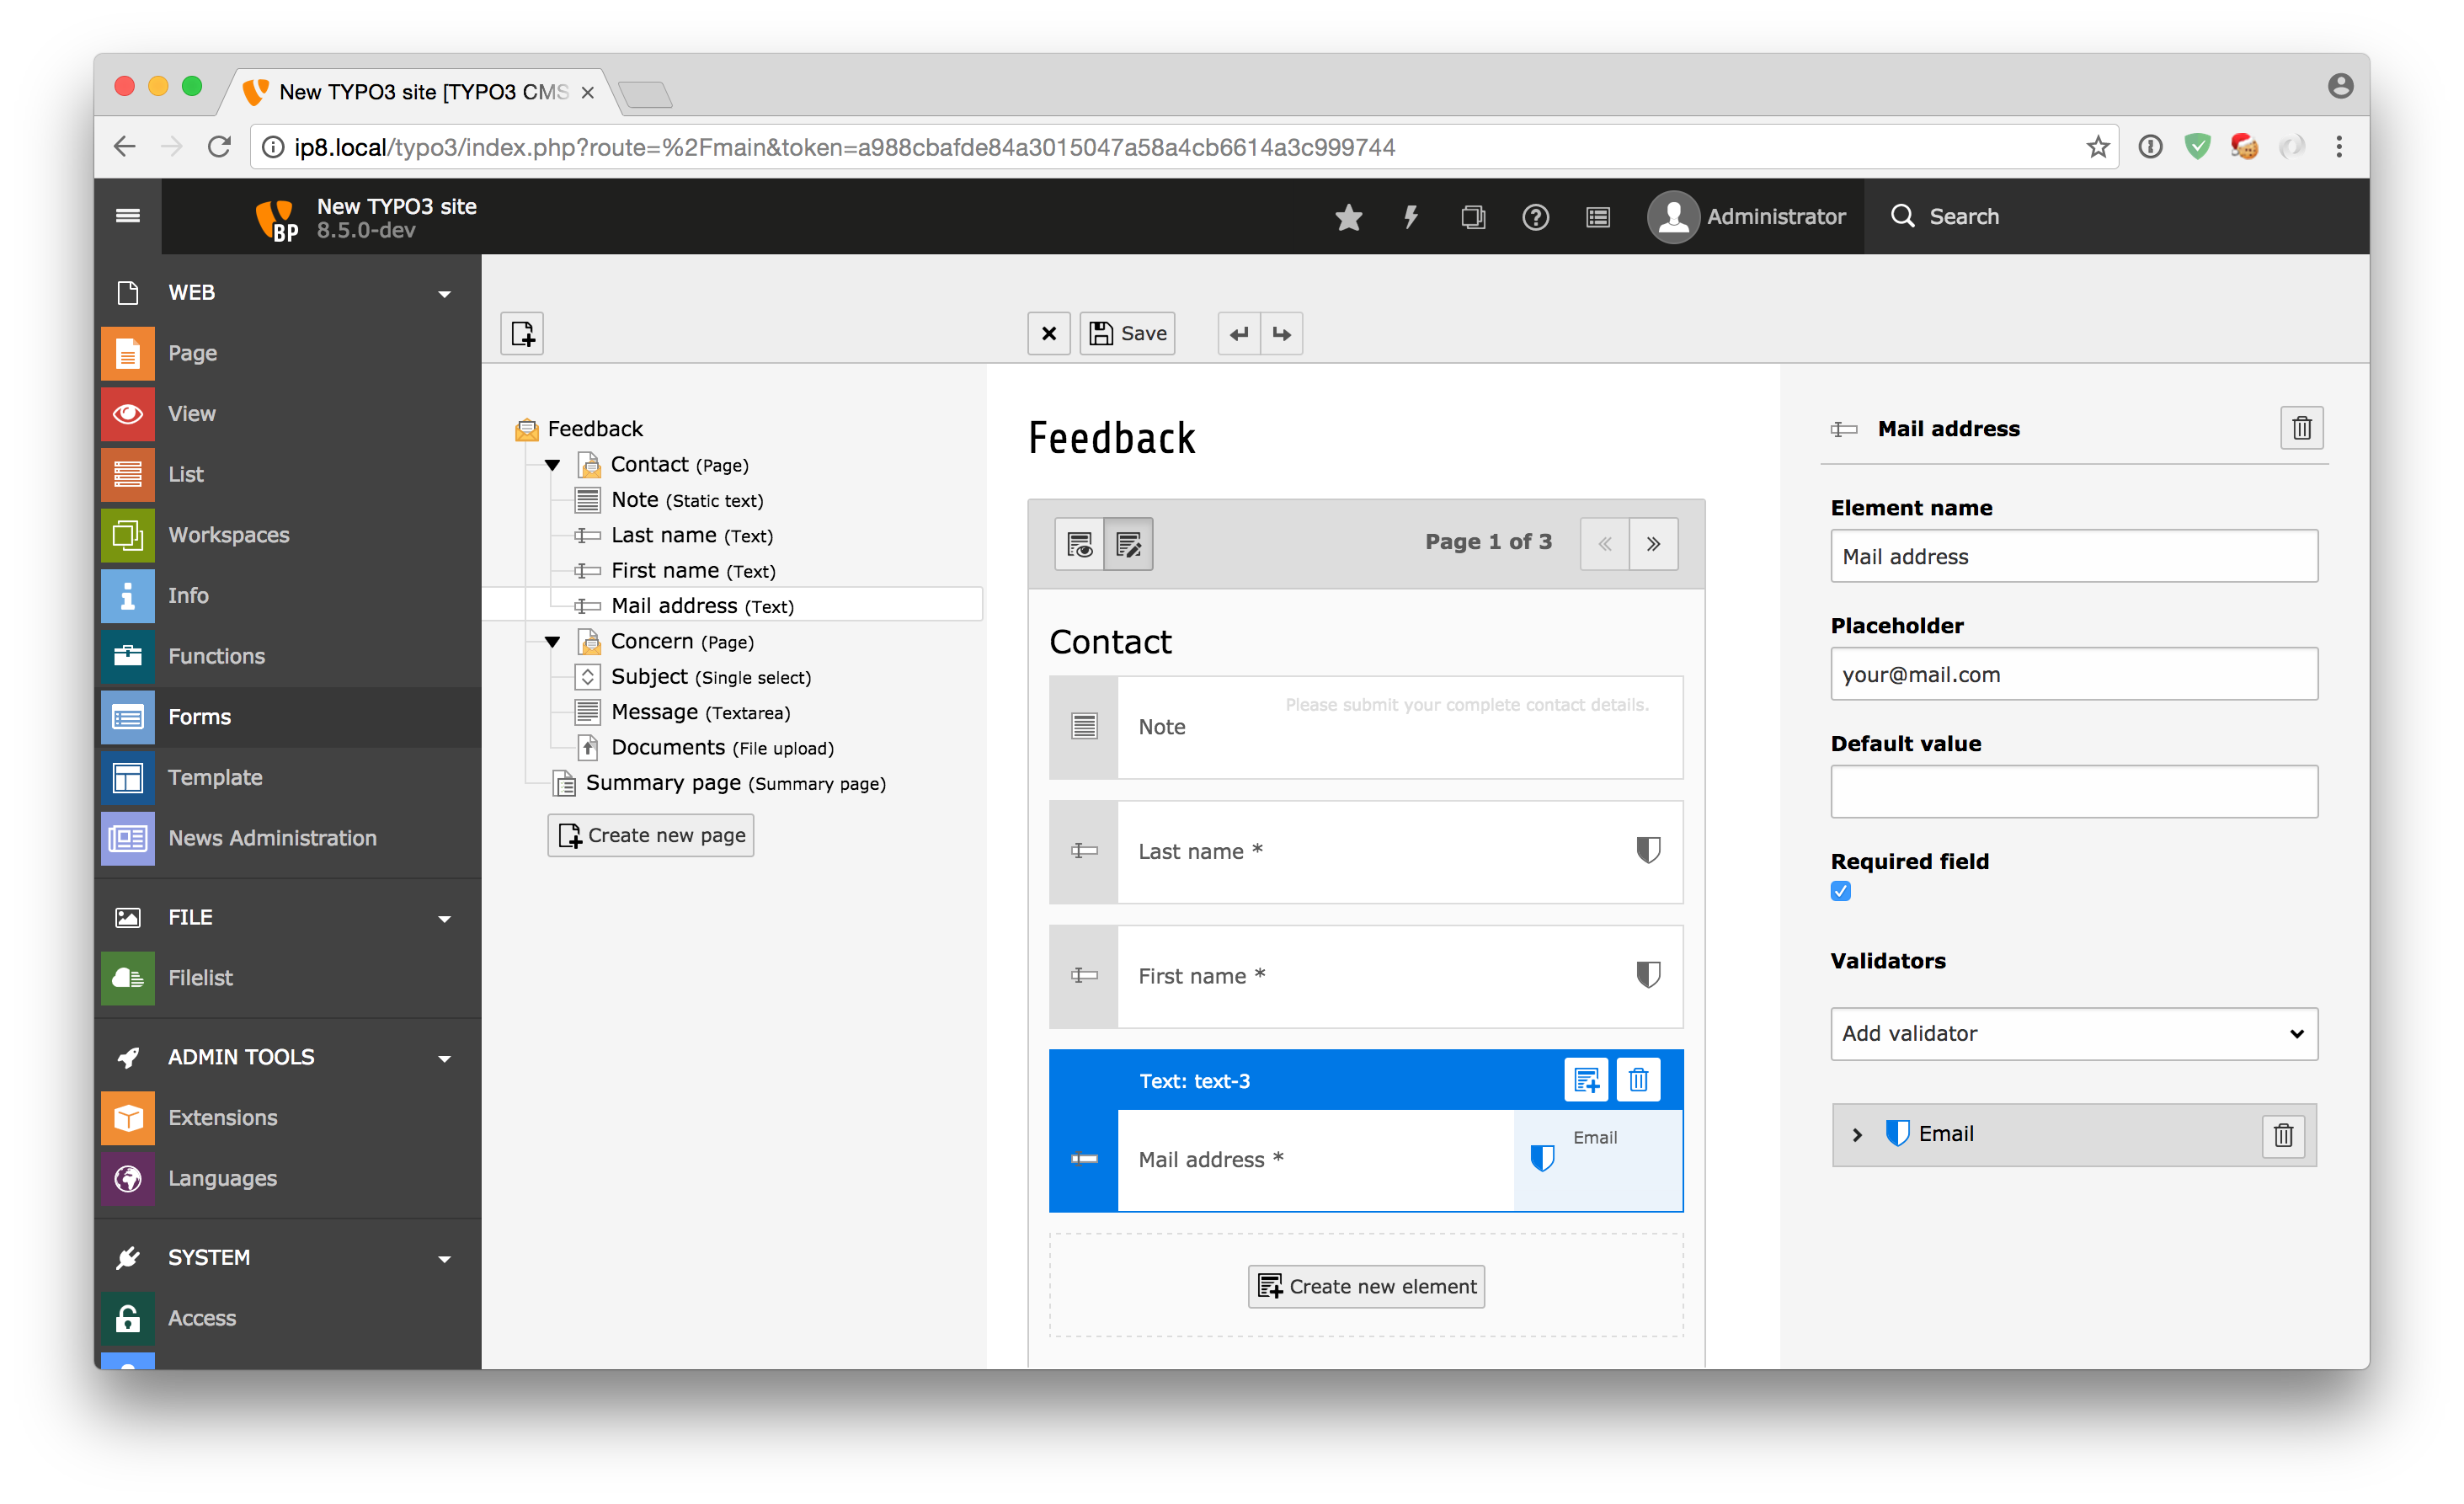
\includegraphics[width=0.8\linewidth]{BackendUserInterface/form-framework-1.png}
	\end{figure}

\end{frame}

% ------------------------------------------------------------------------------
% LTXE-SLIDE-START
% LTXE-SLIDE-UID:		8558dcf2-3966fbad-5b5f954b-a6e69d45
% LTXE-SLIDE-ORIGIN:	b91ec75b-7aa7b566-b523ca5f-f9ba3cde English
% LTXE-SLIDE-TITLE:		#77910: New Form Framework (3)
% ------------------------------------------------------------------------------
\begin{frame}[fragile]
	\frametitle{Backend User Interface}
	\framesubtitle{New Form Framework (3)}

	\begin{figure}
		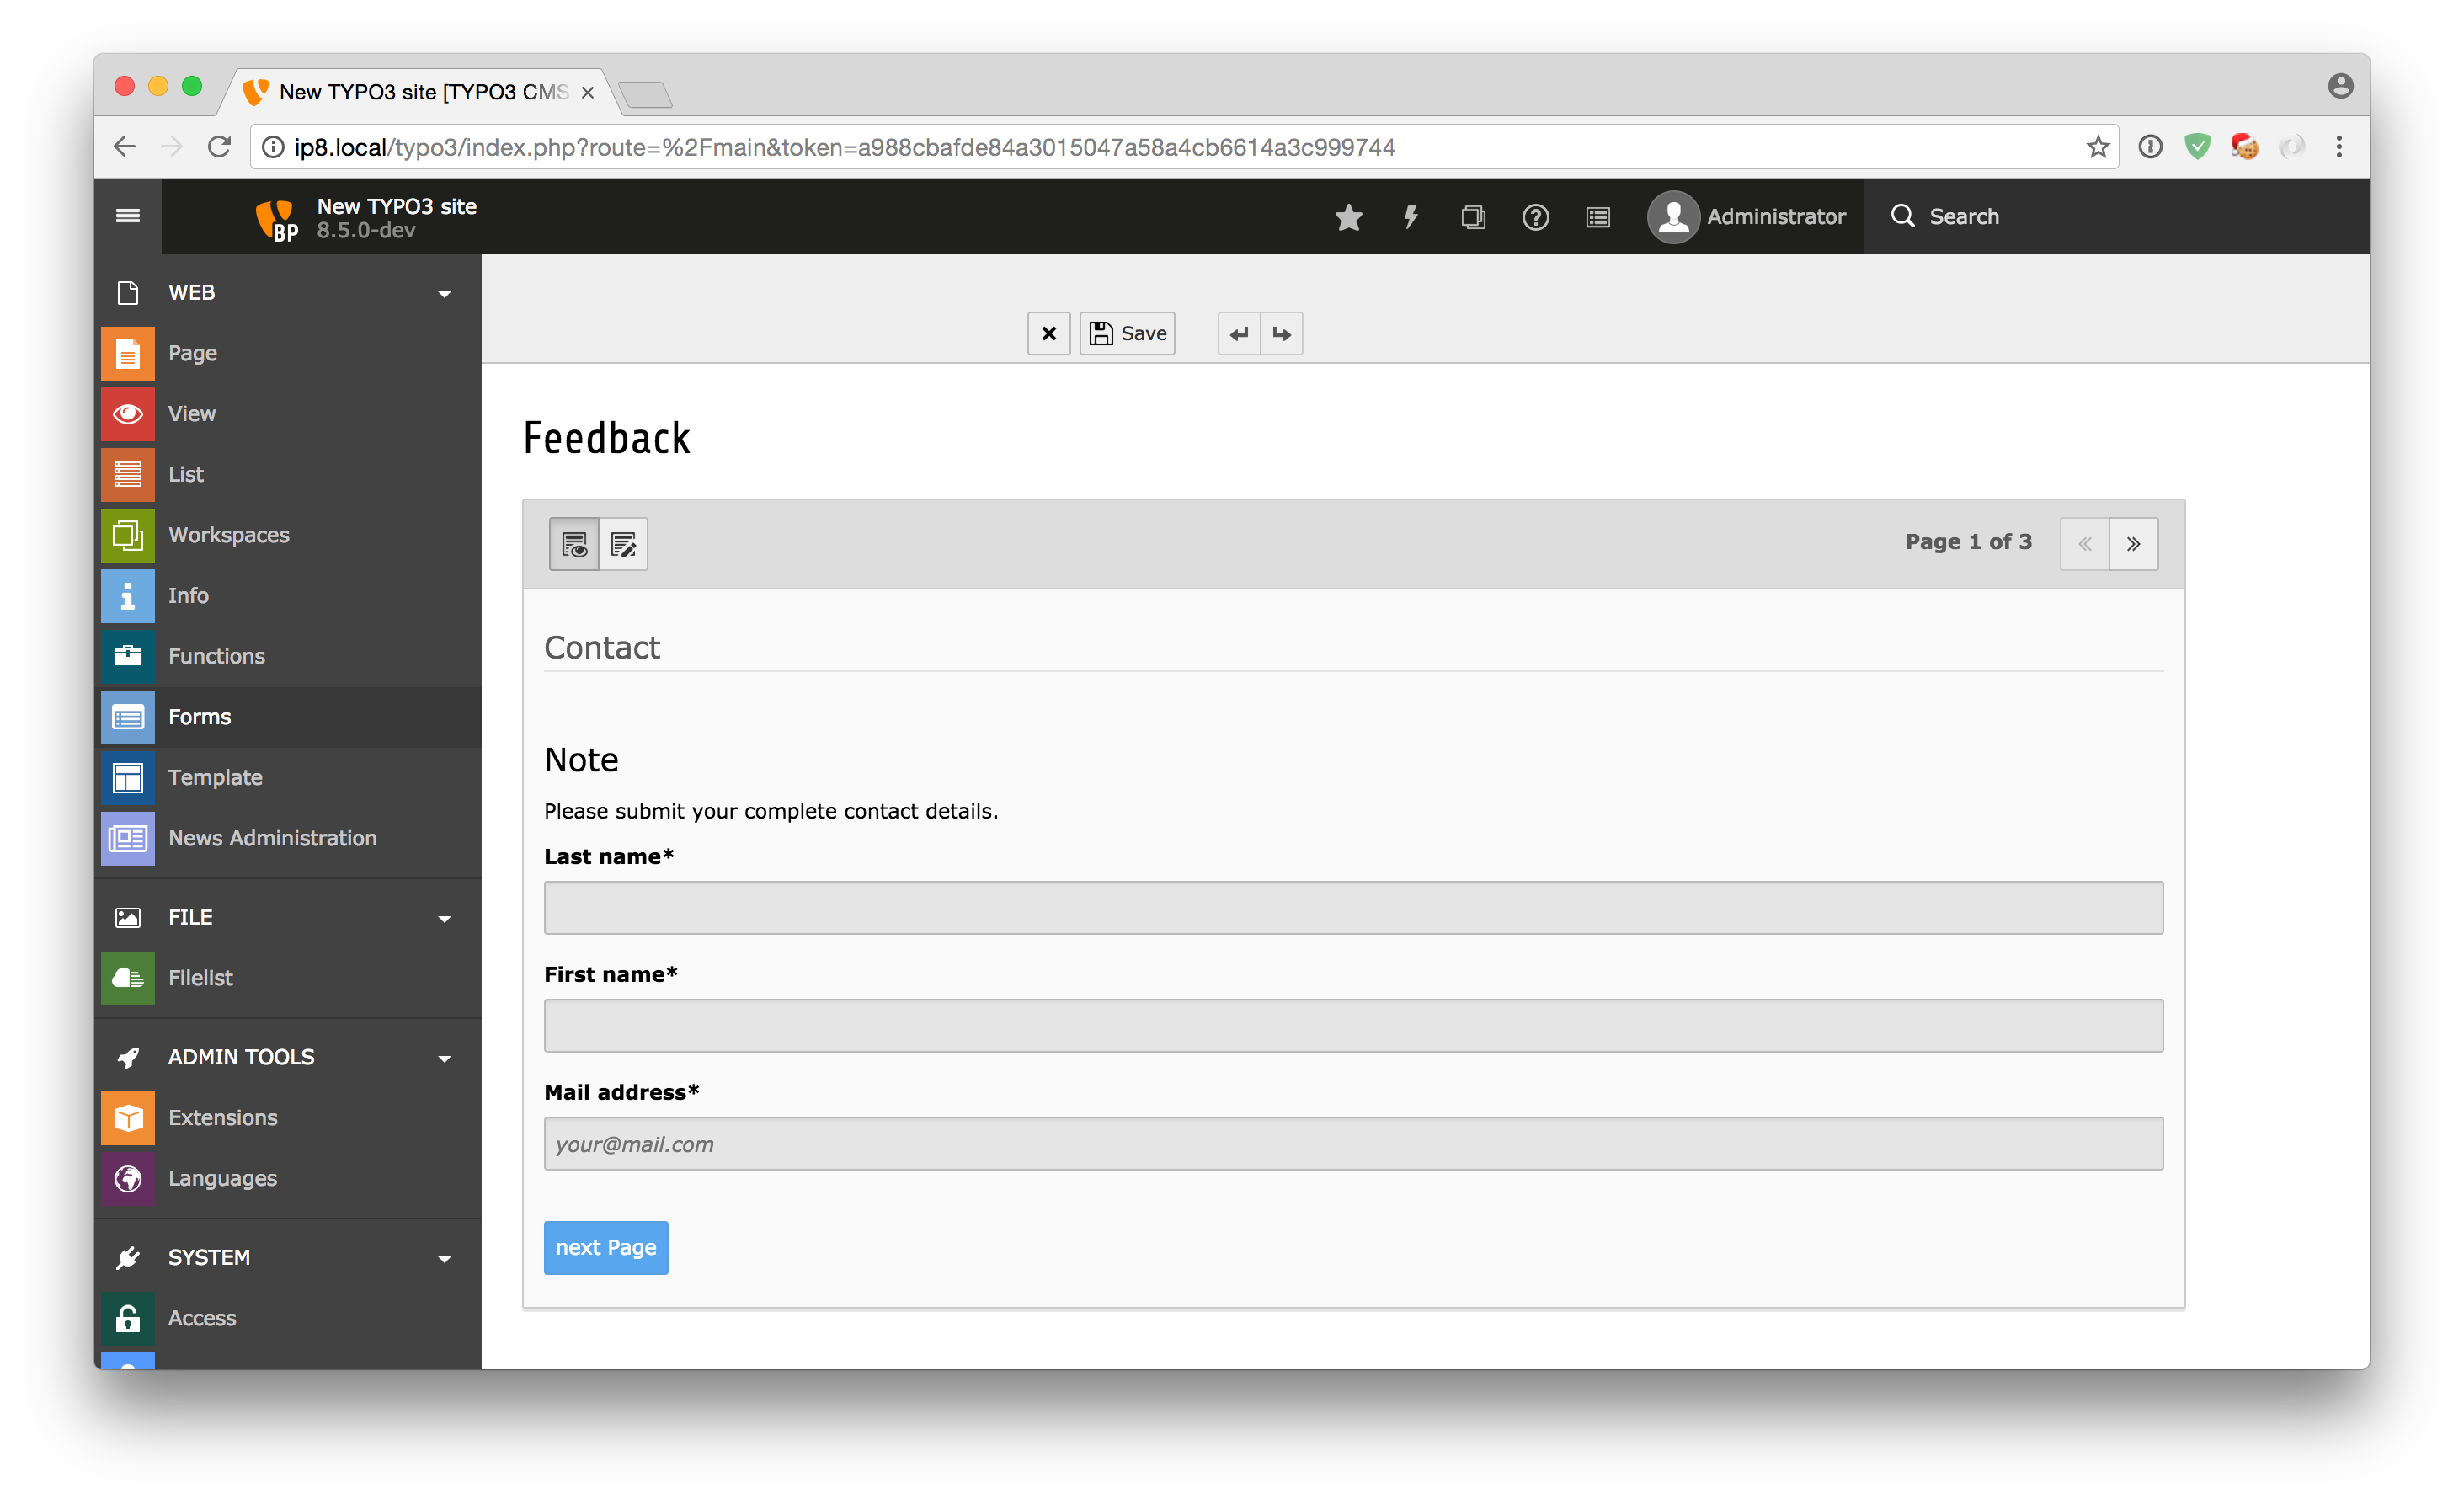
\includegraphics[width=0.8\linewidth]{BackendUserInterface/form-framework-2.png}
	\end{figure}

\end{frame}


% ------------------------------------------------------------------------------
% LTXE-SLIDE-START
% LTXE-SLIDE-UID:		bb749c2c-41013543-2fd4bdf6-8757612a
% LTXE-SLIDE-ORIGIN:	c41b2f21-fb92bb80-56e7ddc9-1c725e34 English
% LTXE-SLIDE-TITLE:		CKEditor Integration
% ------------------------------------------------------------------------------
\begin{frame}[fragile]
	\frametitle{Backend User Interface}
	\framesubtitle{CKEditor Integration}

	\begin{columns}[T]
		\begin{column}{.5\textwidth}
			The next generation of rich text editing has been implemented in the TYPO3 backend:
			\textbf{CKEditor}.\newline

			The current state is explicitly marked as \textit{experimental} and the extension
			is not installed by default.\newline

			Further details about this open source editor: \url{http://ckeditor.com}
		\end{column}
		\begin{column}{.5\textwidth}
			\begin{figure}\vspace*{-0.4cm}
				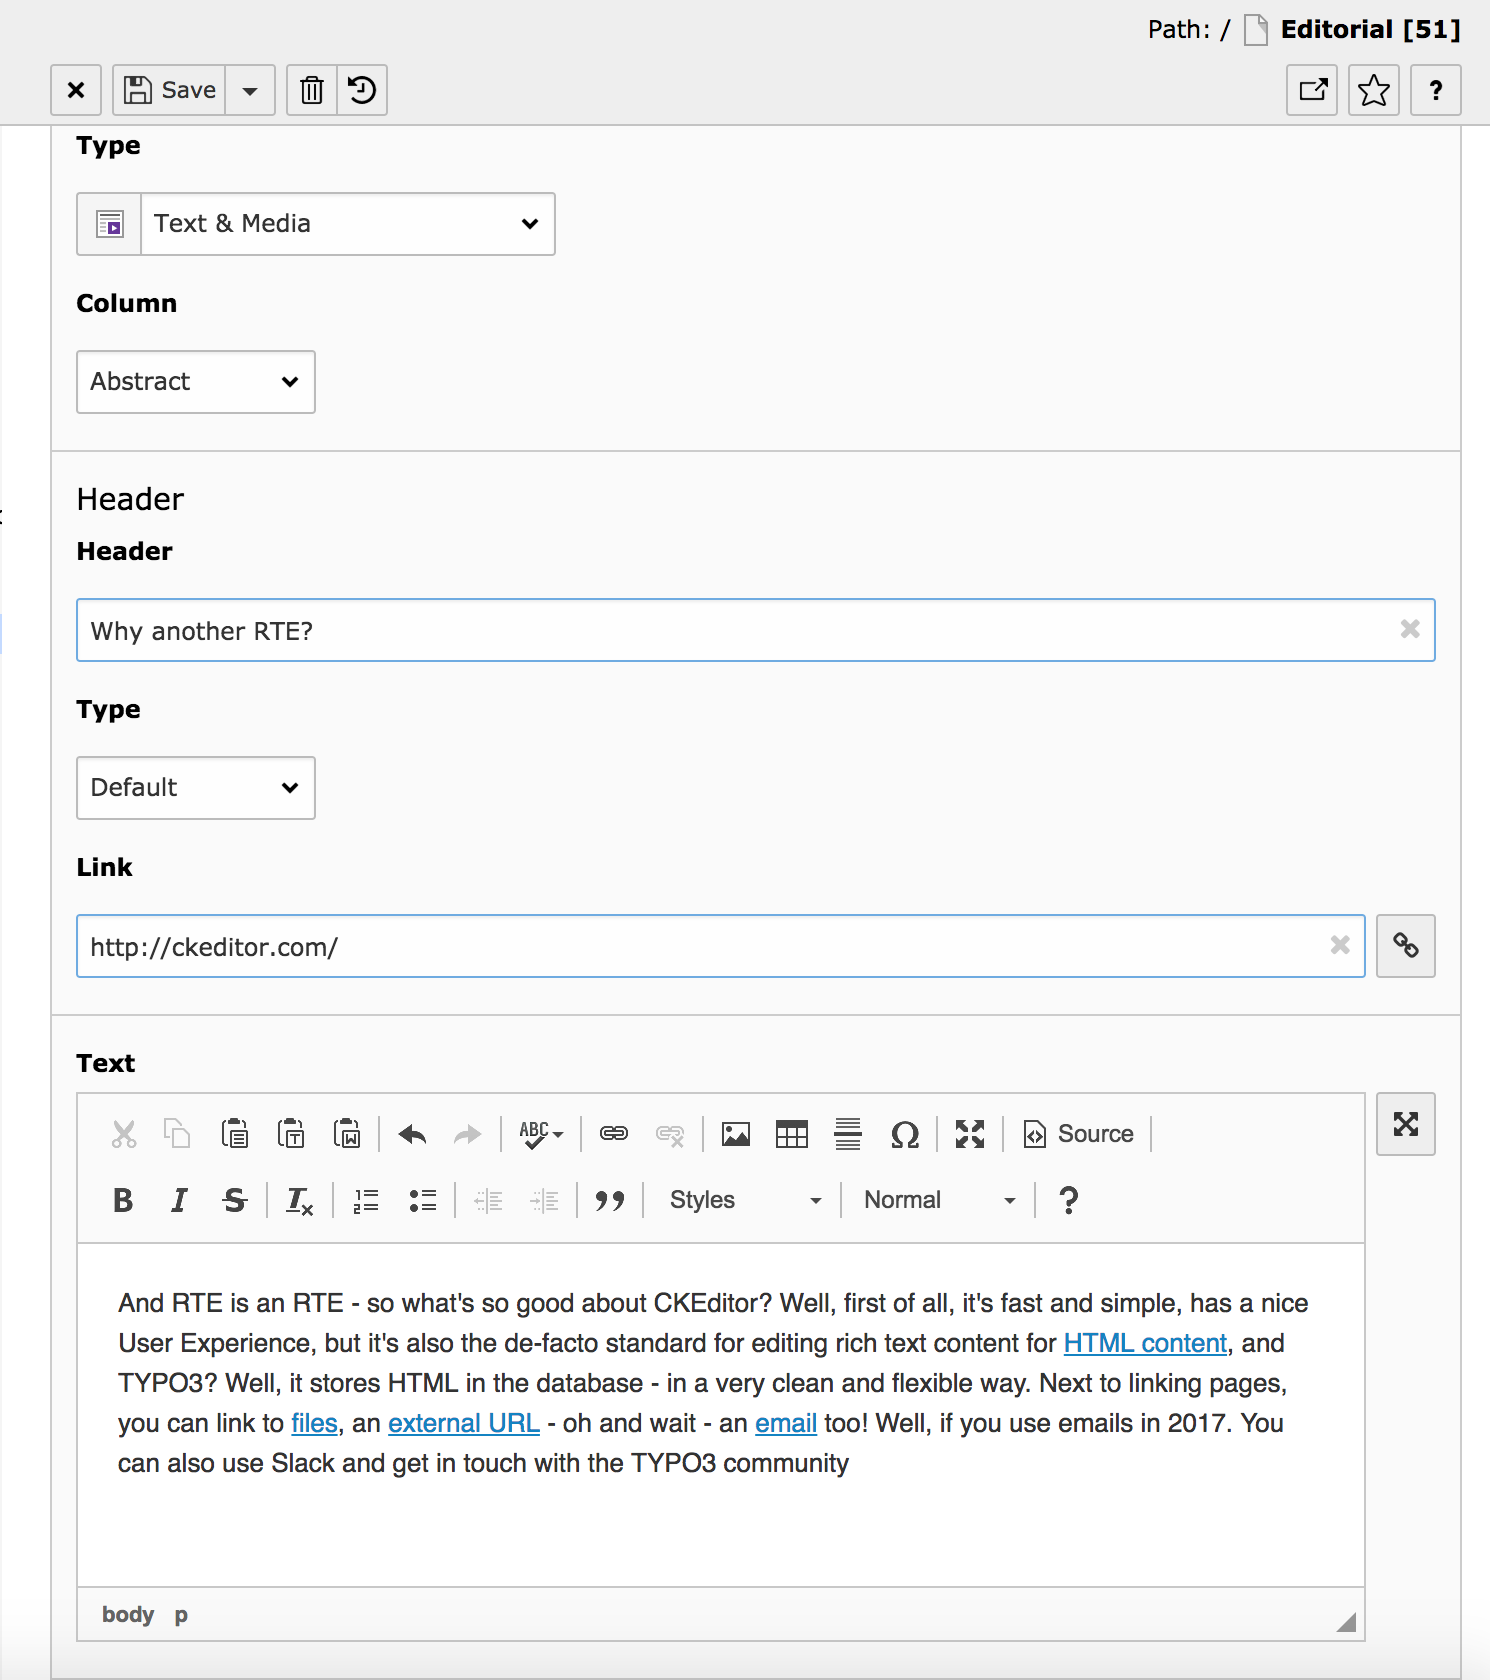
\includegraphics[width=0.8\linewidth]{BackendUserInterface/ckeditor.png}
			\end{figure}
		\end{column}
	\end{columns}

\end{frame}



% ------------------------------------------------------------------------------
% LTXE-SLIDE-START
% LTXE-SLIDE-UID:		b5e42dcb-0bddd03b-c6e3d218-603744af
% LTXE-SLIDE-ORIGIN:	c9dc360d-cf218f95-03f53731-03d821ad English
% LTXE-SLIDE-TITLE:		#78383: Field positions in tabs streamlined (TCA)
% ------------------------------------------------------------------------------
\begin{frame}[fragile]
	\frametitle{Backend User Interface}
	\framesubtitle{Position and Order of Elements}

	\begin{itemize}
		\item The order and position of certain fields in the backend of TYPO3 has been streamlined
		\item The aim is to meet users' expectation where to find commonly used options in the user interface
		\item This is especially important for recurring field definitions and generic categories shared by a lot of records
		\item Extension authors are encouraged to follow the specified positions and orders of elements in
			the \href{https://docs.typo3.org}{official documentation}

			% TODO: update link above (waiting for Doc and Core Team to finish documentation)

	\end{itemize}

	\begin{itemize}
		\item \textit{Backend consistency is king!} :-)
	\end{itemize}

\end{frame}

% ------------------------------------------------------------------------------
